 \documentclass[compsoc, 10, draftclsnofoot, onecolumn]{IEEEtran}
\usepackage{listings}
\usepackage{underscore}
\usepackage[bookmarks=true]{hyperref}
\usepackage[utf8]{inputenc}
\usepackage[english]{babel}
\usepackage{indentfirst}
\usepackage{hyperref}
\usepackage{color}
\usepackage{tikz}
\usepackage{rotating}
\usepackage{pgfgantt}
\usepackage{xcolor}
\usepackage{graphicx}

\definecolor{barblue}{RGB}{153,204,254}
\definecolor{groupblue}{RGB}{51,102,254}

\newganttchartelement{orangebar}{
    orangebar/.style={
        inner sep=0pt,
        draw=red!66!black,
        very thick,
        top color=white,
        bottom color=orange!80
    },
    orangebar label font=\slshape,
    orangebar left shift=.1,
    orangebar right shift=-.1
}

\newganttchartelement{bluebar}{
    bluebar/.style={
        inner sep=0pt,
        draw=purple!44!black,
        very thick,
        top color=white,
        bottom color=blue!80
    },
    bluebar label font=\slshape,
    bluebar left shift=.1,
    bluebar right shift=-.1
}
\newganttchartelement{greenbar}{
    greenbar/.style={
        inner sep=0pt,
        draw=green!50!black,
        very thick,
        top color=white,
        bottom color=green!80
    },
    greenbar label font=\slshape,
    greenbar left shift=.1,
    greenbar right shift=-.1
}

\renewcommand\thesection{\arabic{section}}
\renewcommand\thesubsection{\arabic{section}.\arabic{subsection}}

\hypersetup{
    %bookmarks=false,    % show bookmarks bar?
    pdftitle={Kite Software Requirements},    % title
    pdfauthor={David Baugh, Andrew Bowers, Sawyer Kokesh},% author
    pdfkeywords={requirements documents, Capstone, Kite}, % list of keywords
    colorlinks=true,       % false: boxed links; true: colored links
    linkcolor=blue,       % color of internal links
    citecolor=black,       % color of links to bibliography
    filecolor=black,        % color of file links
    urlcolor=blue,        % color of external links
    linktoc=page            % only page is linked
}%
\urlstyle{same}
\def\myversion{ 1.0 }
\date{}

\usepackage{hyperref}
\title{Kite : A Social Media Journal App}
\author{ %not author the sponsor
	Project Sponsored By: \\
    David Vasquez
}

\begin{document}
\null  % Empty line
\nointerlineskip  % No skip for prev line
\vfill
\let\snewpage \newpage
\let\newpage \relax
\maketitle
\begin{center}
\huge{The Preliminary Design Document}\par
\vspace{2mm}
\large{Written by:}\par
\normalsize{David Baugh}\par
\normalsize{Sawyer Kokesh}\par
\normalsize{Andrew Bowers}\par
\vspace{8mm}
\large{\textbf{Abstract:}}\par 
\vspace{2mm}


\normalsize{This Software Design Document provides an in-depth look at how the Kite project plans to design and implement a social media application. This document aims to describe how the different components will be designed during application development. Furthermore this document gives a outline of how the Kite application was created for use by future developers.} 

\end{center}
\let \newpage \snewpage
\vfill 
\break % page break

\tableofcontents
\newpage

\section{Overview}
\subsection{Introduction}
This document aims to describe the Kite project from different viewpoints while also breaking down how each viewpoint will be solved. With each viewpoint the overall project is viewed in a smaller scope allowing for a more in depth look at the implementation of the challenges and elements that relate to that specific viewpoint. The document also provides a stable reference for the development team to reference when communicating about different features of the application. A well thought out and agreed upon design document will help deliver a streamlined and cohesive Kite application.   

\subsection{Scope}
This document will cover how the Kite application will be developed during the 2017-2018 school year. Portions of the application will be broken down into viewpoints, where each viewpoint is different, and described. The scope of the this document only covers the required features, which does not include the stretch goals of the project. In other words the features that are designed and described in this document are the agreed upon deliverables that are to be completed by expo.

\subsection{Purpose}
In the world filled with social media and online entertainment, lives are posted online 255 characters at a time, sometimes with a picture for good measure. Not one social media site is a complete solution for every person and thus leaves some without a way to express themselves online. This application aims to solve this by providing a more in-depth story driven posting experience. The purpose of the Kite project is to design and create this in-depth journal-like experience within the Kite app, a social media journaling community.

%Must include Definitions
\section{Definitions and Abbreviations}
\begin{enumerate}
\item \textbf{Kite: } Name of the project and related mobile app.
\item \textbf{Event: } A grouping of entries of a span of time i.e. "Vacation" or "Senior Year".
\item \textbf{Community: } A public profile that allows Kite users to post entries on a communal page.
\item \textbf{Tags: } A "hashtag" or a "\#" is used to relate a journal entry to a topic, such as \#football, or \#funny. A "at" tag or "\@"is used to relate a user with a journal entry, in this case a user will be sent a notification each time that user is tagged in a journal entry. Tags might also be used to correlate event comments to their specific entry within said event
\item \textbf{Moderator: } User with the permissions to edit and change a community's page.
\item \textbf{Admin: } User with the permissions to delete any user and post on the Kite application.
\item \textbf{Entries: } A single post from one user onto the Kite application.
\item \textbf{Journal: } A journal is a collection of a user's or community's entires.
\item \textbf{UI: } An abbreviation for User Interface.
\end{enumerate}

\section{Conceptual Model for Software Design Descriptions }
\subsection{Software Design in Context}
The decision to develop a mobile application rather than a web browser was made with the growing application market in mind. Application development for mobile devices is very popular, primarily due to the increased use of mobile devices in everyday life. People use their mobile devices to schedule their day, pay bills, and communicate with others and now, with the Kite application, they can tell a story about an event that has happened or is happening in their life. The mobile platform option offers more users for both general use as well as during testing while the application is being developed. 

\subsection{Software Design Decisions within the Life Cycle}
Decisions regarding the basic hardware and platforms to be used are essential points of the Kite project. The Kite project will initially be developed for both iOS and Android mobile platforms with a web based platform as a stretch goal. To accomplish this goal, the team has decided to design the project using React Native. This mobile development language is supported by both iOS and Android and also allows for drop in Objective-C and Java. One of the other major decisions will be in user interface design. To ensure the user interface is moving in the right direction during development, the Kite team will be using paper prototyping and live models to test initial interface designs as well as working designs.    

\section{Mobile Language Viewpoint}
\subsection{Design Elements and Information} For the project, as noted in the "Software design decisions within the life cycle" section, the Kite project will be using React Native for mobile application development. This language utilizes React libraries while using Javascript as its framework. One of the major factors in choosing this language was its ability to support both iOS and Android Development allowing for more users as well as a larger testing pool. The language will allow for a larger user testing pool as well as more users, in a general sense, for the application.

\subsection{Design Concerns} One of the main concerns with using React Native for this project is its slightly steep learning curve and it being a newer language. Although there are several very good resources to use for trouble shooting and learning or using this language, the number of good sources is still less than that of Objective-C or Java. The Kite group will rely on the React Native resource page as well as a few other notable sources for assistance in the use of the language. 

\section{Context Viewpoint}
\subsection*{Design Concerns}
The Kite app will be used in the context of a user adding or viewing different posts that they or other users have created. There are many different concerns when designing the Kite app for a user in this context. The first concern is allow each user the ability to log into and out of the app. Once a user can get access to their profile the users next concern will be to set up or change the setting of their account. Once this has been done, the User may want to first view other people's journal entries, this can be done a number of ways, either looking at the discover page or searching for journals. If the user sees a journal that they want to look at more closely, they can click on it and view it. The user may also see that some of the items on the discover page are events, when these are clicked on they can see a list of many journals that relate to this event. This user can also create their own journal entries or events. The user can also follow other users, this allows the user to view their timeline page. The timeline page is populated with posts from users that this user follow.

\subsection*{Design Elements}
\paragraph*{Login/Logout}
The Login page is a simple page that will allow for a user to log into their account and see all of their information. This allows the User to login from different devices, or change what account they are login as. To logout they just simply have to click on the menu dropdown button and click logout, this will allow them to get back to the Login page to change Users.
\paragraph*{Profile}
The User Profile is a page that contains informations about the login in User. This information can be viewable by other user if the permissions are set up to allow this.
\paragraph*{Discovery}
The Discovery page is the main way that the user will see new Users Journal entries. This is a random selection of posts that are viewable in a scrollable list. 
\paragraph*{Searching}
When the User knows what they are looking for they are able to use a simple search option, the search can only find other Users. This search option allows the User to quickly find other users when they know there name.
\paragraph*{Journal}
A Journal is created by User to share their experiences in terms of text and embedded photos. A Journal entry can only be edited by the user that has created it. Once a Journal is created and viewable to others, it can be liked and commented on. 
\paragraph*{Event}
A User can create an Event, a Event is a collection of Journal that relate to defined time interval. Scene this is a collection of Journals, the Event also has a running total of likes. Similarly to Journals the event itself can also be commented on.
\paragraph*{Timeline}
The Timeline will be different for each User, it is a random collection of Journals that have been created by users that this User is currently following. This is like the Discovery page with a filter for Users that are being followed by this User.

\section{Information Viewpoint}
\subsection{Design Elements}
The Kite application is mostly data driven, in other words, the main action that will occur when using this app is uploading and retrieving data. One of the primary features of the application is enabling users to upload profile pictures as well as edit their profile with personal information. Beyond the user profile, users can also create posts, which can be anything they want them to be. The posts give users the opportunity to share a story, or event, something going on in their life with much more detail. Posts allow users to categorize their information using Events. To describe this briefly, say, for example, if a user had a hiking trip over a span of several days. The user could then make posts using this Event as a means to organize their posts, as well as any of the pictures or videos uploaded. Categorizing and organizing this information allows the users who make the original post to have more control of how their content will look as well as allow other users viewing the content to have more control over what they are seeing. 

\subsection{Data Storage Viewpoint}
\subsubsection{Data Manipulation}
PHP is the main way that app will communicate with the database. The first thing that needs to happen to connect the app with the database is to create the configuration to the database. Within the app, a fetch method can be called which intern will run the PHP script. Within the fetch method, a JSON string can be constructed with information which is then sent to the PHP script. Within the PHP script, the JSON string will be converted into a object. Within the PHP, a SQL query will be created to insert or gather information from the database. If the data is posted to the database, the PHP will then just return either an accepting or error text. If the query is getting data from the database, then the PHP will return what the query returned. This provides the necessary connection between the Kite application and the database.

\section{Interface Viewpoint}
\subsection{Interface Elements}
The Kite user interface will consist of a many different frameworks and components to create the user interaction model. The overall navigational framework of Kite will be used to move from page to page within the application, such as the timeline and profile pages. The design of each of the different frameworks and pages within the application will be built with long term use and user interactivity in mind.

\subsubsection{Navigation}
The navigation of the Kite application must allow users to move about the application and find the options or content that they want at that time. The combination of a tab bar near the bottom of the screen, and a hamburger menu near the top of the screen will be the main components of the navigational system. These two menu elements will contain every main page and option for the Kite application. The lower tab bar will contain the pages that are going to be cycled through on a regular basis. These pages will potentially contain the timeline, communities, notifications, profiles, and journals. The hamburger, or 3 bar menu, in the upper left of the screen will contain every other option and page available to the user. Those other options will contain the security settings, settings in general, and additional options the user might need to make their experience even better.
\begin{center}
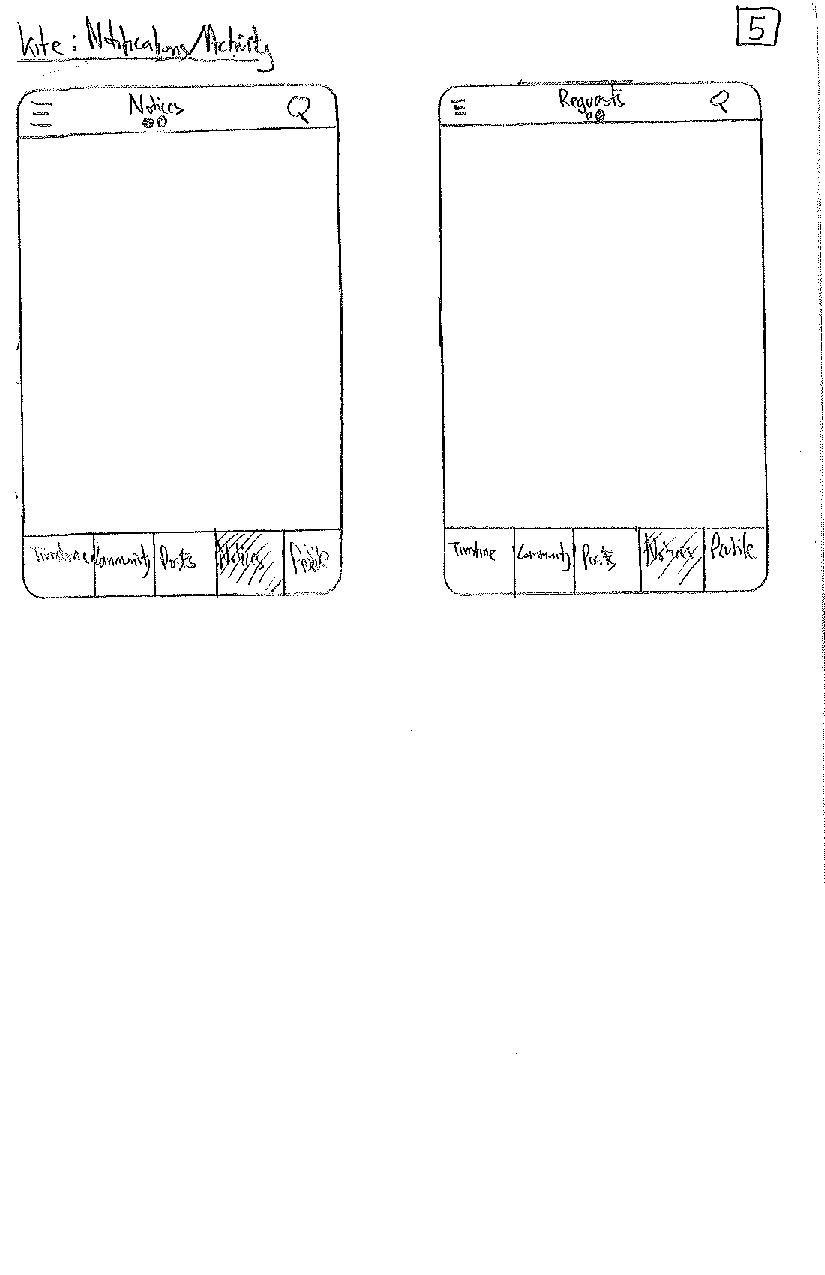
\includegraphics[width=0.5\textwidth]{Notifications}

An early Navigation layout draft 
\end{center}

\subsubsection{Timeline}
The timeline will be the main source of content for the user. This page will, like many other social media applications, be where friends, followers, and other user's public journal entries will show up per the user's social settings. The page will be a scrollable flow of the journal entires. The ability to like, comment on, and maybe share a journal entry will be available with each entry and event. This page should allow a user to enjoy scrolling through what could be an extensive amount of information that is in front of them. The layout needs to allow the user to distinguish between the individual entries and events. The UI will allow the user to access more information about the specific entires they are reading whether that be more about the user or the date it was written on.
\begin{center}
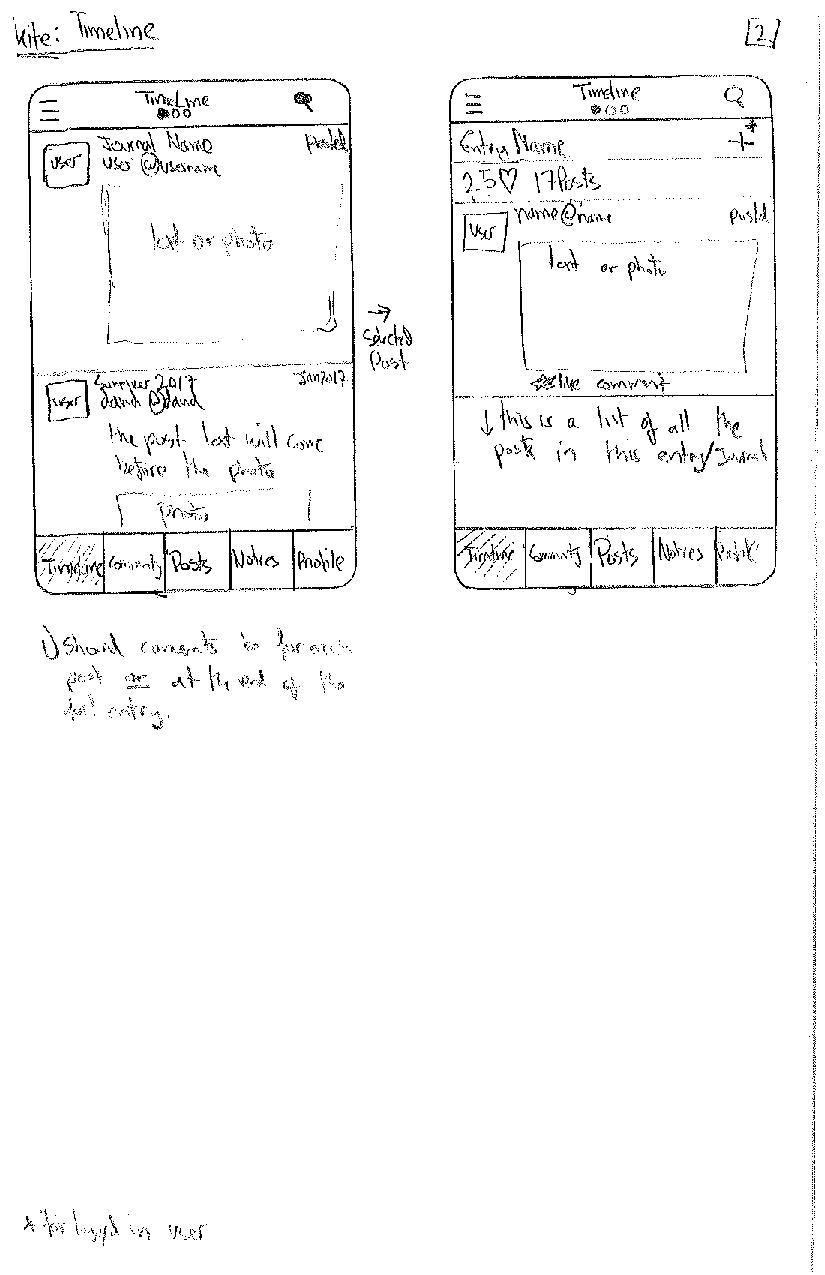
\includegraphics[width=0.5\textwidth]{Timeline2}

An early draft of the Kite timeline
\end{center}

\subsubsection{Communities}
Much like the timeline page, communities are pages of scrolling content for the user to cycle through. The major difference between the user's main timeline and communities is that communities will be focused on a single main subject such as a place or public figure. These communities will allow like-minded users to come together and share their thoughts in a safe and secure location. A community will have, in addition to a common subject, more moderation. The creator of a community is given administrator control over the running of the community. The admin will also have to ability to give community users moderator powers. These mods will then oversee the community and keep the community members accountable to the rules set by the administrator within the context of that community. Communities will allow people come together and share their adventures and thoughts on subjects in which they share with their peers. The communities must be able to support an administration hierarchy and more settings options relating to the privacy of the entries and events posted within the community's page.  

\subsubsection{Events}
Events are a collection of journal entries. The format of events will allow users to take a collection of vacation or diary entires and combine them into a single collection. The event will have a single title with an abstract summary which will be what is shown on a user's timeline instead of the entire contents of the entires within it. While each entry within will still retain its own likes and comments, the event will add up all of the likes and collect the comments into a single space. Users will also be able to comment on the entire event as a whole instead of a single entry. Potentially tags could be used within the commenting system to signify which comments belong to which entry within the event but that is part of the project's stretch goals
\begin{center}
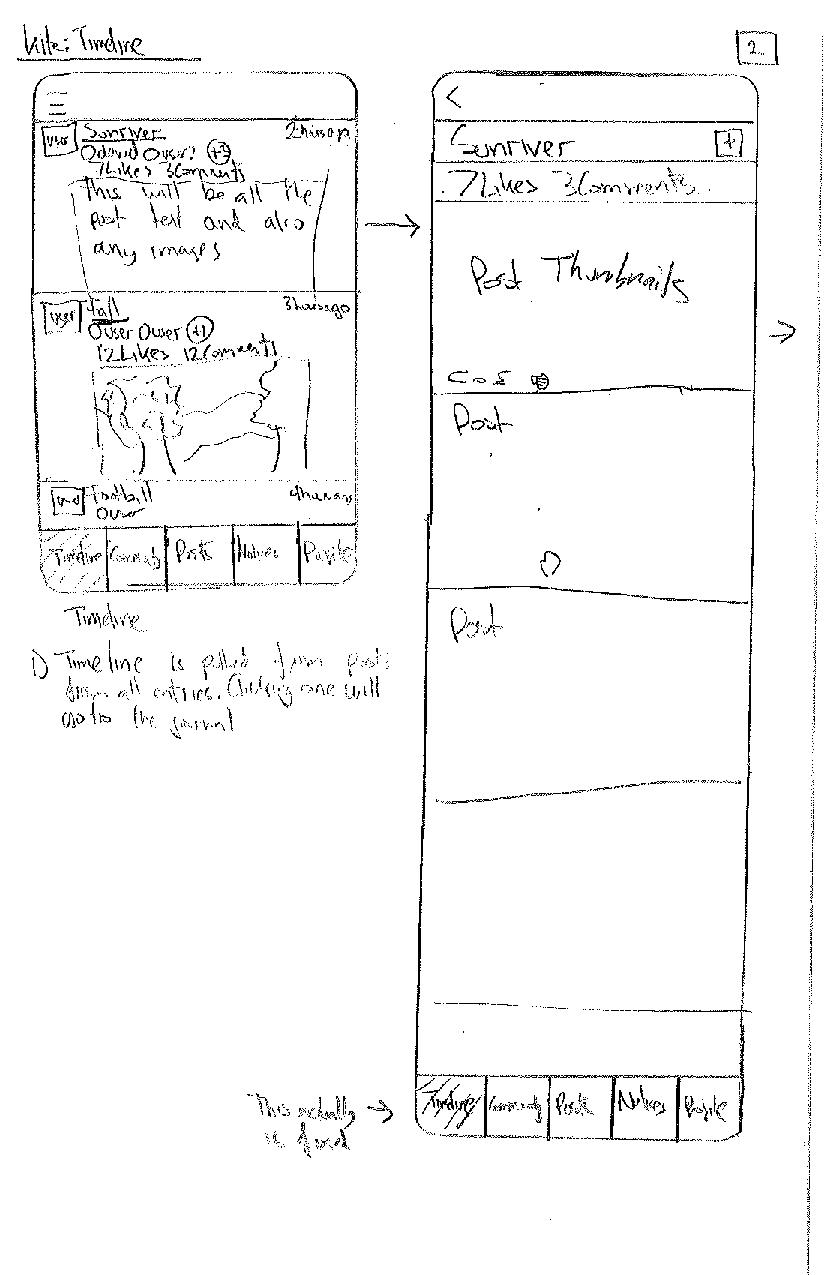
\includegraphics[width=0.5\textwidth]{Timeline}

An extended view of the event 
\end{center}

\subsubsection{Notifications}
The Notification page will be the page where any sort of update or invite Kite thinks the user needs to see will be updated with said content. Each individual notification will be linked to the content it represents and wants the user to see so that the user can instantly go to the page and view the content it was asked to view. 

\subsubsection{Profile}
The profile page contains the personal information of a Kite user. If the page is the user's personal profile page, the page will contain settings to edit their personal information and to view what the user has posted recently. If the page is of another user's profile, then the page will simply be viewable but not editable. The page will show a user's followers, posts, communities, and more. All information that the user has set to be public will be available on their profile page. 
\begin{center}
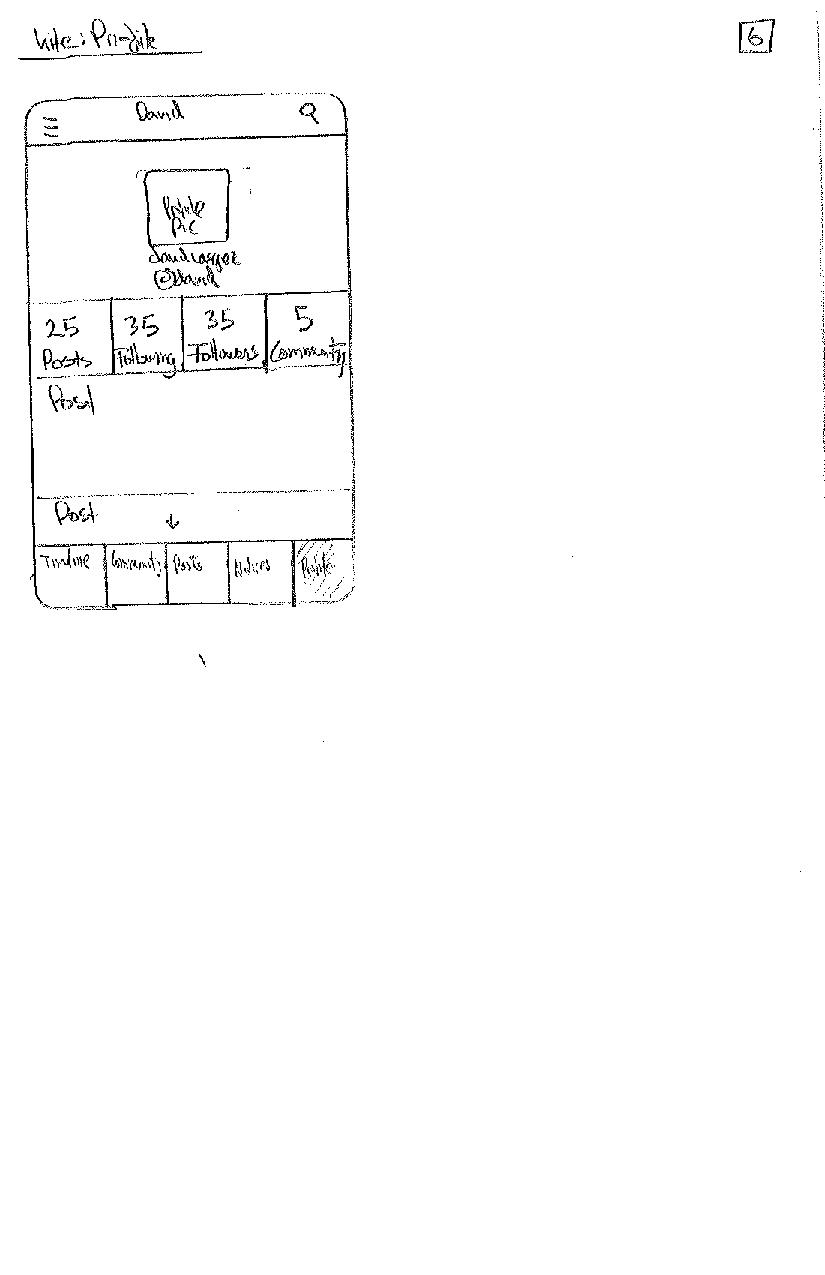
\includegraphics[width=0.5\textwidth]{Profile}

A profile page early draft
\end{center}

\subsubsection{Log-in/Register}
This page will allow the user to log into their personal account or to register and create an account of their very own. The page will be very basic as to focus the user's attention on the selectable options of login and register. The page itself will be used in a very limited capacity as it will be used only once at the beginning of each session when a user activates Kite for use.
\begin{center}
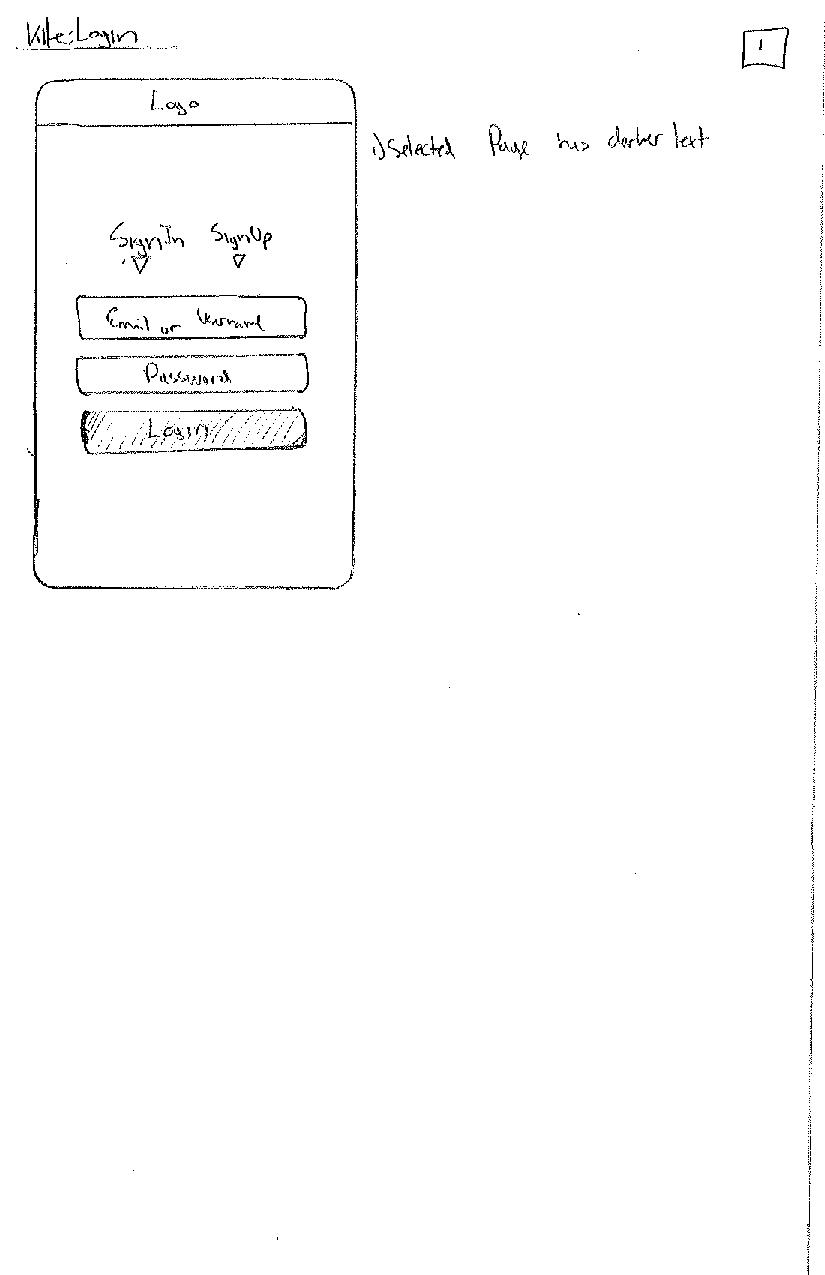
\includegraphics[width=0.5\textwidth]{Login}

An early look at the Kite login screen
\end{center}

\subsection{Interface Testing} The Kite application aims to have a fluid easy-to-use interface that supports its story driven purpose. To do this, the application interface will be tested using both Android and iOS users to ensure a similar quality experience for each user. To provide this level of quality, user testing through paper prototyping, or UI mock-ups drawn on paper, will be held early on in development. Paper Prototyping will enable test users to simulate using the application, thus allowing the Kite developers to gather information on areas the user finds problematic. Beyond initial prototype testing, user tests will be run throughout the development of the user interface using device emulators and actual android and iOS devices.

\subsection{Interface Concerns} One of the main problems involved with the development of the interface for the Kite application is the trouble of offering the same quality and user experience between both mobile platforms being developed for. Android makes use of built-in buttons, either hardware or on-screen software, to navigate applications, whereas iOS typically makes use of on-screen gestures, like swipes or buttons. There are more differences between iOS and Android that will need to be taken into account when developing this app. One of these differences is that Android is open source and iOS is not. Because of this problem, there maybe many developers contributing to the improvement of this operating system. With Android being open source, it may be more vulnerable to security issues and bugs that iOS might not have. On the other hand, iOS is closed source; because of this, only Apple developers are able to create, update, and fix iOS. This can end up being more secure in some cases, but making the OS closed source means that the iOS applications such as Apple Maps, Mail, and Safari are exclusive to the iPhone. iOS is in contrast with Android in which all of their apps are open to the iPhone as well. Allowing our application to be written in React Native, Kite will be available to as many hands as are possible which is a necessary requirement for a social media application.     

\subsection{Interface Structure}
As stated in section 3.2, the language that the Kite project will be developed in will be React Native. Components are how React Native divides up the screen into individual sections; each viewable part of the screen will be a separate component. There are a few simple design decisions that will be implemented for the React Native structure of the user interface. The first is to keep each component as simple as possible. When each component is simple, it becomes much easier to add or change features within a single page. Another design decision that is important is to keep the navigation separated from the individual views. A component can hold multiple smaller views within it. This will be beneficial when moving the navigation out of the view to be controlled by the component so each view does not have to keep track of navigation. Each page has a set of components that give the app a more connected feel when navigating. When an application does not have a cohesive style it feels more clunky and disjointed to navigate through which could hinder usability.

\newpage
\section{Kite Project Timeline}
\subsection{Timeline Gantt Chart}
\begin{rotate}{270}
\begin{ganttchart}[
    hgrid style/.style={black, dotted},
    vgrid={*5{black,dotted}, *1{white, dotted}, *1{black, dashed}},
    x unit=.8mm,
    y unit chart=9mm,
    y unit title=12mm,
    time slot format=isodate,
    group label font=\bfseries \Large,
    link/.style={->, thick}
    ]{2017-10-04}{2018-06-21}
    \gantttitlecalendar{year, month=name}\\

    \ganttgroup[
        group/.append style={fill=orange}
    ]{Kite App}{2017-10-04}{2018-4-5}\\ [grid]
    \ganttorangebar[
        name=Documentation
    ]{Documentation}{2017-10-07}{2017-12-20}\\ [grid]    
    \ganttorangebar[
    	name=Database
    ]{Database}{2017-11-01}{2018-01-10}\\ [grid]   
    \ganttorangebar[
    	name=App Design
    ]{App Design}{2017-11-01}{2018-02-30}\\ [grid]    
    \ganttorangebar[
    	name=User Interface
    ]{User Interface}{2017-12-01}{2018-4-05}\\ [grid]
    \ganttorangebar[
    	name=Networking
    ]{Networking}{2017-11-01}{2018-01-10}\\ [grid]
    
    \ganttgroup[
        group/.append style={fill=blue}
    ]{Test Cases}{2018-01-10}{2018-05-01}\\ [grid]
    \ganttbluebar[
        name=Database
    ]{Database}{2018-01-10}{2018-02-15}\\ [grid]
	\ganttbluebar[
        name=User Interface
    ]{User Interface}{2018-02-30}{2018-05-01}\\ [grid]
    
    \ganttgroup[
        group/.append style={fill=green}
    ]{Expo Prep}{2018-05-01}{2018-06-15}\\ [grid]
    
\end{ganttchart}
\end{rotate}
\newpage
\subsection{Timeline Description} This timeline is the outline of the expected time for the Kite development team to develop each of the sections. The project has been split up into three main section  Kite App development, Test Cases, and Expo Prep. The Kite App development section is the largest part of the Kite project because this is were the main framework is coded as well as styled. Moreover this section is where most of the documentation is going to be written up. The next section is the Test Cases, this section is going to used to go though the app and see if it works as the requirements state. If it does not match this is were we will update and change the app as well as update the documentation to make sure all of the requirements have been met and are working. The only new documentation that will be added in this section of working will be testing documentation. The last section is Expo Prep, this will be the shortest section in terms of time. This time is going to be spent polishing up our app. The Expo Prep time will be also spent creating the expo poster for the Kite app as well as creating a demo to show at the expo, and finally to get the expo presentation walked though and cohesive. The Timeline spans from the beginning of fall term and ends at the end of spring term.   

\section{Conclusion}
Over the course of the 2017 to 2018 academic year, the Kite development team will first start the database for the data storage as well as developing UI mock ups and begin  paper testing. Networking and security will go hand in hand and will developed together. Followed closely after, will be finalizing the application and continue on-device testing to polish the final product for the Engineering Expo. During this time period, user testing will continue throughout ranging from on paper to on-device testing. As well as client and TA meetings to keep the project moving forward, correctly, and in a timely manner. Version 1.0 will be completed and ready for the Engineering Expo where the Kite application will be available for viewing and exposition.
  
\newpage
\end{document}